\documentclass[draft]{article}

\usepackage{fancyhdr}
\pagestyle{fancy}
\usepackage{pdfpages}
\usepackage{graphicx}
\usepackage{amsmath}
\usepackage{listings}
\lstset{columns=fullflexible, basicstyle=\scriptsize\sffamily}

\lhead{Simon}
\rhead{ECE 3710}

\title{Simon Design Document}
\author{ Aaron Yardley, Mark Li}
\date{12/9/2016}

\setlength{\parskip}{1em}

\begin{document}

\sloppy
\maketitle
\newpage
\tableofcontents
\listoffigures
\pagenumbering{gobble}
\newpage
\pagenumbering{arabic}



\section{ Introduction}
\par
The purpose of this document is to describe the design of a memory game similar to the game Simon Says.  The document contains hardware, software, and logic design on how we built this project.
\par
\noindent
Simon is a memory game in which the microcontroller creates a pattern for the user to input. Once the pattern is generated, 
the user repeats the pattern by inputting the corresponding button.  All patterns are generated randomly.  When the user has input 
an incorrect pattern, then the game is over and the high score is saved.

\section{Scope}
\par
\noindent
This	document	discusses	in	detail,	the	electrical	and	software	design of Simon.	It	includes	requirements,	dependencies	and	the	theory	of	operation.	Hardware	
schematics	and	code	for	the	project	are	included	for	a	more	thorough	explanation	of	the	
design.	Testing	Procedures	and	results	of	each	requirement	are	included.		

\section{Design Overview}
This section will describe the requirements, dependencies, and the theory of operations.
\subsection{Requirements}
 \begin{enumerate}
   \item There will be nine segments to display that are all separate colors.
   \item There will be ten sounds outputed to a speaker using a DAC: 1 sound per button, and a game over.
   \item The beginning pattern will have three randomly generated buttons to output.
   \item The pattern produces one new random button to be saved to the pattern.
    \item The speed will increase for the output of the pattern as the game continues.
   \item The high score must be saved through power resets.
  \item There must be an animation to show a game over.
  \item There will be a timer between button sampling that if it times out the user loses.
  \end{enumerate}

\subsection{Dependencies}
The following items are required in order for the hardware  and software to run properly.
\begin{enumerate}
\item 5 volt source to power the DAC and LCD touchscreen.
\item 3.3 Volt source to power the microcontroller and the LCD touchscreen.
\item 16 Mhz external crystal for the source clock.
\item Reset switch.
\item TM4C123GH6PM chip.
\item WaveShare 320x240 3.2" Resistive Touchscreen TFT LCD, using ILI9341 LCD and XPT2046 Touch Screen
\item 12-bit AdaFruit DAC (using MCP4725)
\item Analog Test Board Speaker with LM386M amplifier
\end{enumerate}

\subsection{Theory of Operations}
When reset switch is hit, the screen prints the high score and the nine buttons.  This is followed by showing the initial pattern consisting of
three random squares.  These squares are black out and then filled in to show that this button has been selected.  The game then waits for
the user to input the same pattern.  If the user correctly inputs the pattern, then the pattern is again displayed with an additional random square.  This continues until the user incorrectly enters the pattern.  The incorrect pattern immediately is followed by an animation of the screen followed by the output of game over.
\par
\noindent
The score is set by how many buttons you have in the last pattern minus one.  If the current score is higher than the current high score, the high score is updated.  The high score should be saved by using non-volitile memory so that when a power reset happens the high score is saved.  

\section{Design Details}
This section is used to descrbe the hardware and software of the project.
\subsection{Hardware Design}
This section describes the LCD Touchscreen and Digital to Analogue converter(DAC).
\subsubsection{LCD Touchscreen}
In order to realize the game, we worked with the LCD and the touchscreen independent from each other.  We used the display screen to display a three by three set of buttons each represented by a different color.  At the top of the screen we will display the high score of the game so players have an opjective while playing.  The touchscreen is used to recieve user input for the game.  The pin layout is described in Figure 1.

\subsubsection{DAC with Speaker}
We two pins for the I2C communication.  The I2C signal sends a digital signal to a DAC to create a sine wave to output on the speaker.  In order to create a smoother sound and a more ideal sine wave we added a capacitor in series with the speaker.  This is shown if figure 2.

\subsection{Software Design}
This section describes the software of the game.  
\subsubsection{Initializations}
The entire program was realized using a 40 MHz clock.  We used two communication, I2C to communicate with the DAC and SPI communication for the LCD touchscreen.  We had nine different colors to use for each of the buttons so that there wouldn't be any confusion as to which button needed to be pushed.  To realize how to draw letters, numbers, and symbols, we used an array with an offset in ascii of all the ascii characters so when we wanted to draw a character we would pass a function a character and it would draw the character.  
\par\noindent
The last part of the initialization is to create a begining sequence of three buttons.  The random pattern is generated by taking samples of the system clock timer and modulo 9 the value.  We then use the number to correspond with a box on the display.  As described in the theory of operations, once the random pattern is set the screen then blacks out and fills in the box generated by the random code.  Inorder to save this pattern, we save the pattern numbers in an array to compare with when the game has started.  

\subsubsection{Gameplay}
Although not in our requirements, we wanted the user to be able to see where he was touching to ensure that was the button that was intended to be pushed.  After a button was pushed, a sound would be outputted on the speaker to  incorporate sound with each button.  Because the touch screen and LCD cannot get coordinates and output a display simultaneously, we had to create a fast way to display and output a sound to the speaker.  Instead of darkening out the entire box, like the pattern display sequence, we only darkened out a small section of the button to increase the speed of drawing.  Once the touchscreen is released, the actual pattern is compared to the users last input.  If pressed correctly the game continues, otherwise the game ends.  
\par
\noindent
When the initail pattern has been complete, the system clock then is used to create an additional button.  This new button is added to the end of the pattern array.  The array then is outputted on the screen.  The pattern is always saved this way.  
\par\noindent
The end of the game is shown with an animation as well as a buzzer.  The animation that we chose was inverting the screen and turning the screen of and on several times in about two seconds.  This is followed by outputting a "Game OVER!" at the top of the screen.

\subsubsection{Score}
Each game has a score based on the maximum number of correct buttons.  The output of the score was not part of the requirements, but would be easy to include.  If the current score is greater than the existing high score, the new high score is written into flash memory.  This memory in non-volatile, meaning when power is lost during a reset, the data is saved.  The process of reading and writing from flash memory takes a long time compared to writing to SRam.    Because of this, we are only saving one number at the end of the program so that reading and writing this data doesn't affect the rest of the programs speed.  

\section{Testing}
The following section shows the requirement and how they are being met.
\subsection{Requirement 1}
There will be nine segments to display that are all separate colors.
\begin{figure}[h]
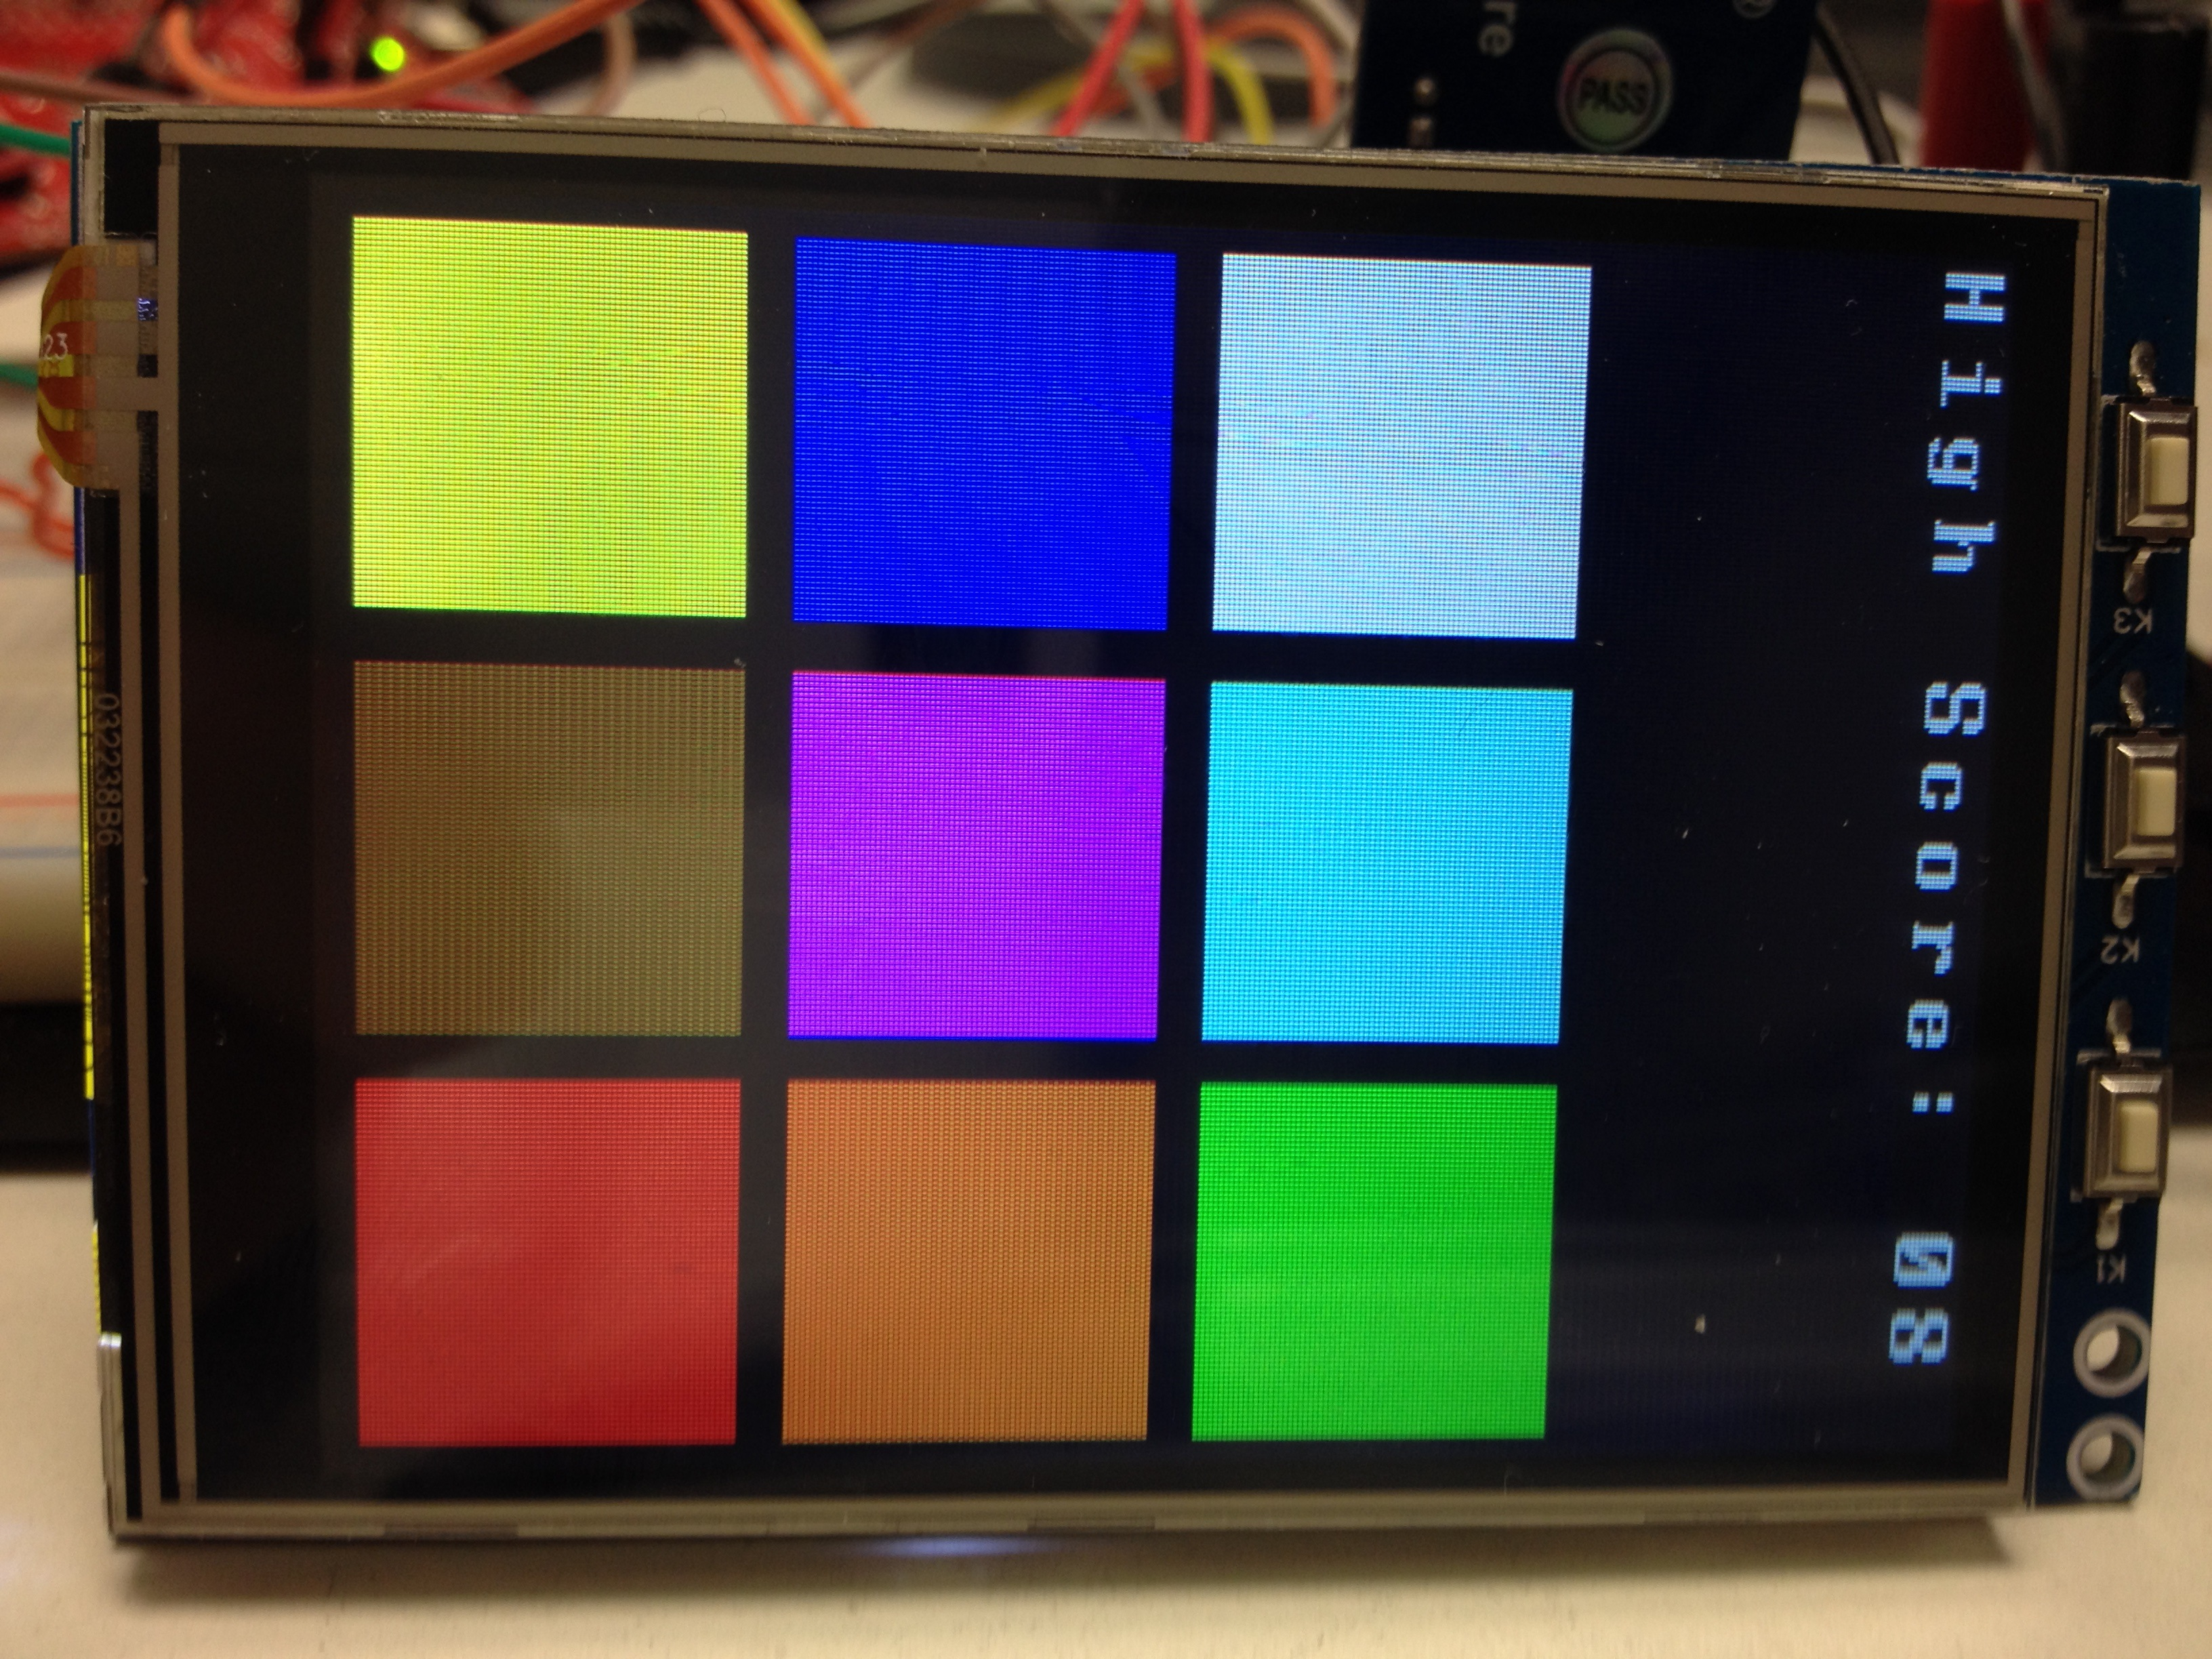
\includegraphics{images/InitialScreen.jpg}
\caption{Initial Game Screen}
\label{Figure1}
\end{figure}
\subsection{Requirement 2}
There will be ten sounds outputed to a speaker using a DAC: 1 sound per button, and a game over.
\subsection{Requirement 3}
The beginning pattern will have three randomly generated buttons to output.
\subsection{Requirement 4}
The pattern produces one new random button to be saved to the pattern.
\subsection{Requirement 5}
The speed will increase for the output of the pattern as the game continues.
\subsection{Requirement 6}
The high score must be saved through power resets.
\subsection{Requirement 7}
There must be an animation to show a game over.
\subsection{Requirement 8}
There will be a timer between button sampling that if it times out the user loses.

\section{Conclusion}
The impementation of the game Simon that we set was successfull by meeting the following requirements.  It allowed a player to be tested and challenged by a memory game.  The LCD touchscreen was a great way to implement the display and touch of the game and reduced addtional hardware.  
\par\noindent
The	design	described	is	a	successful	prototype	with	limited	functionality.	This	design	can	
be	improved	by creating different game modes as well as having the user touching the screen to start the game.	


\end{document}

